\chapter{Présentation du stage}

Le stage a débuté au début du mois de juin 2024. Un ordinateur et un PIN-pad générateur d'OTP (One-Time-Password) ont été mis à ma disposition. Carlos, mon maître de stage, m'a fourni les instructions nécessaires pour comprendre et utiliser Antares\cite{antares}, une librairie de développement, à l'aide de la documentation en ligne\footnote{Documentation d'Antares : https://cerfacs.fr/antares/}.

\section{La librairie Antares}

La structure des solutions CFD interprétées dans Antares est illustrée ci-dessous :

\begin{figure}[ht!]
\centering
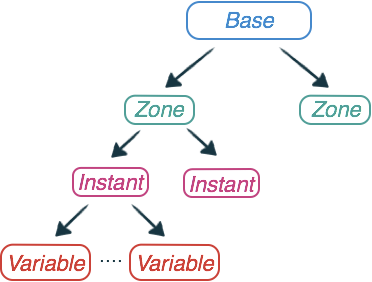
\includegraphics[width=0.5\textwidth]{images/data_structure_1.png}
\caption{Structure des données}
%\footnote{Source:https://cerfacs.fr/antares/src/tutorial/base.html}
%\label{fig:https://cerfacs.fr/antares/src/tutorial/base.html}
\end{figure}

Concrètement, le maillage peut être divisé en plusieurs zones.
Ensuite chaque zone a un ou plusieurs instants où nous pouvons trouver la solution d'une variable, qui sera de même dimension que les coordonnées de l'instant.

Voici un exemple d'utilisation d'Antares :

\begin{lstlisting}[caption=Exemple simple d'utilisation d'Antares pour interpoler, label={lst:antares}]
    import antares
    myt = antares.Treatment('interpolation')
    myt['source'] = source_base
    myt['target'] = target_base
    result = myt.execute()
    print(result[0][0]['v1'])
\end{lstlisting}

Ensuite, la tâche consistait à résoudre un bug mineur sur Antares, ce qui a permis de se familiariser avec Nitrox, le Gitlab hébergé sur le serveur du CERFACS où sont situés Antares et d'autres codes du CERFACS.


\section{Les différentes méthodes d'interpolation}

L'interpolation consiste à déterminer la valeur de nouveaux points à partir de la valeur de points existants. En voici un exemple en une dimension (l'axe x représente la position et l'axe y la valeur des points).

\vspace{0,5cm}


\begin{center}
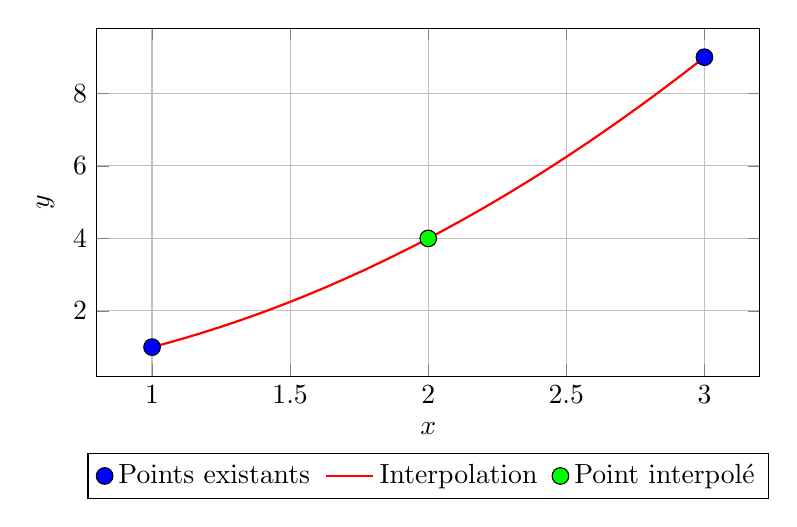
\begin{tikzpicture}
    \begin{axis}[
        width=10cm,
        height=6cm,
        xlabel={$x$},
        ylabel={$y$},
        grid=major,
        legend style={at={(0.5,-0.22)}, anchor=north, legend columns=-1},
    ]

    \addplot[
        only marks,
        mark=*,
        mark options={scale=1.5, fill=blue},
    ] coordinates {
        (1, 1)
        (3, 9)
    };
    \addlegendentry{Points existants \hspace{0,3cm}}

    \addplot[
        domain=1:3,
        samples=100,
        smooth,
        thick,
        red,
    ] {x^2};
    \addlegendentry{Interpolation \hspace{0,3cm}}

    \addplot[
        only marks,
        mark=*,
        mark options={scale=1.5, fill=green},
    ] coordinates {
        (2, 4)%(1.7, 2.89)
    };
    \addlegendentry{ Point interpolé}

    \end{axis}
\end{tikzpicture}
\end{center}

\vspace{0,5cm}

Nous allons premièrement présenter les types d'interpolation implémentables dans Antares, à savoir, qui permette de l'interpolation 3D, sur des maillages dits non structurés, c'est-à-dire pas de simples maillages, rectangulaires en 2D et hexaédrique en 3D, représentés par des matrices, mais des maillages créés avec différentes formes géométriques.
Le temps de calcul, appelé 'coût' est aussi un paramètre à prendre en compte.
Finalement, les caractéristiques mathématiques des équations à interpoler est probablement le paramètre le plus important à prendre en compte, mais aussi assurément le plus difficile. Effectivement différentes équations très difficiles à caractériser mathématiquement tel que l'équation de Naviers-Stokes sont utilisées et le niveau en maths est trop élevé pour pouvoir se plonger en profondeur dans ce problème. C'est pour cela qu'il n'y aura pas de résultat mathématique à présenter dans cette partie. Mais heureusement que ces méthodes ont déjà été implémentés et testés pour d'autres codes de simulation numérique, ce qui donne une bonne idée des résultats que nous pouvons espérer.

%\addcontentsline{toc}{section}{L'interpolation et l'aéroacoustique}

\subsection{L'interpolation par voisin le plus proche}
Cette première méthode est très simple : nous prenons comme valeur \( v \) d'interpolation au point \( p \) la valeur \( v \) du point le plus proche de \( p \).
En voici une illustration :

\vspace{0.5cm}

\begin{center}
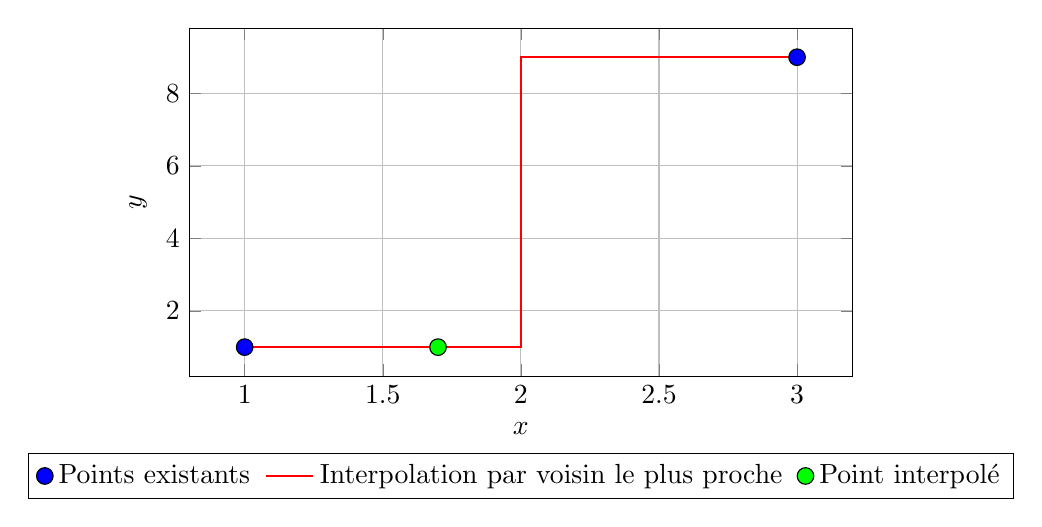
\begin{tikzpicture}
    \begin{axis}[
        width=10cm,
        height=6cm,
        xlabel={$x$},
        ylabel={$y$},
        grid=major,
        legend style={at={(0.5,-0.22)}, anchor=north, legend columns=-1},
    ]

    \addplot[
        only marks,
        mark=*,
        mark options={scale=1.5, fill=blue},
    ] coordinates {
        (1, 1)
        (3, 9)
    };
    \addlegendentry{Points existants \hspace{0,3cm}}

    \addplot[
        thick,
        red,
    ] coordinates {
        (1, 1)
        (2, 1)
        (2, 9)
        (3, 9)
    };
    \addlegendentry{Interpolation par voisin le plus proche \hspace{0,3cm}}

    \addplot[
        only marks,
        mark=*,
        mark options={scale=1.5, fill=green},
    ] coordinates {
        (1.7, 1)
    };
    \addlegendentry{Point interpolé}

    \end{axis}
\end{tikzpicture}
\end{center}

\vspace{0.5cm}

Cette méthode est discontinue et peu précise pour la plupart des fonctions.



\subsection{L'interpolation \ac{IDW}} % déjà '\ac'

Probablement l'interpolation la plus simple après la méthode du voisin le plus proche (toujours dans notre cas d'application), cette méthode est la seule qui étais implémenté dans Antares. Elle a pour formule :

\[
\hat{f}(x) = \frac{\sum_{i=1}^{N} \frac{f(x_i)}{d(x, x_i)^p}}{\sum_{i=1}^{N} \frac{1}{d(x, x_i)^p}}
\]

où :

- \(\hat{f}(x)\) est la valeur interpolée à la position \(x\),

- \(f(x_i)\) est la valeur connue aux points de données \(x_i\),

- \(d(x, x_i)\) est la distance entre \(x\) et \(x_i\),

- \(p\) est le paramètre de puissance,

- \(N\) est le nombre total de points de données.

Pour éviter une division par 0, très proche d'un point existant, le point interpolé prendra la valeur du point existant.
\vspace*{0,5cm}

En voici une illustration :

\vspace{0.5cm}

\begin{center}
\begin{minipage}{0.45\textwidth}
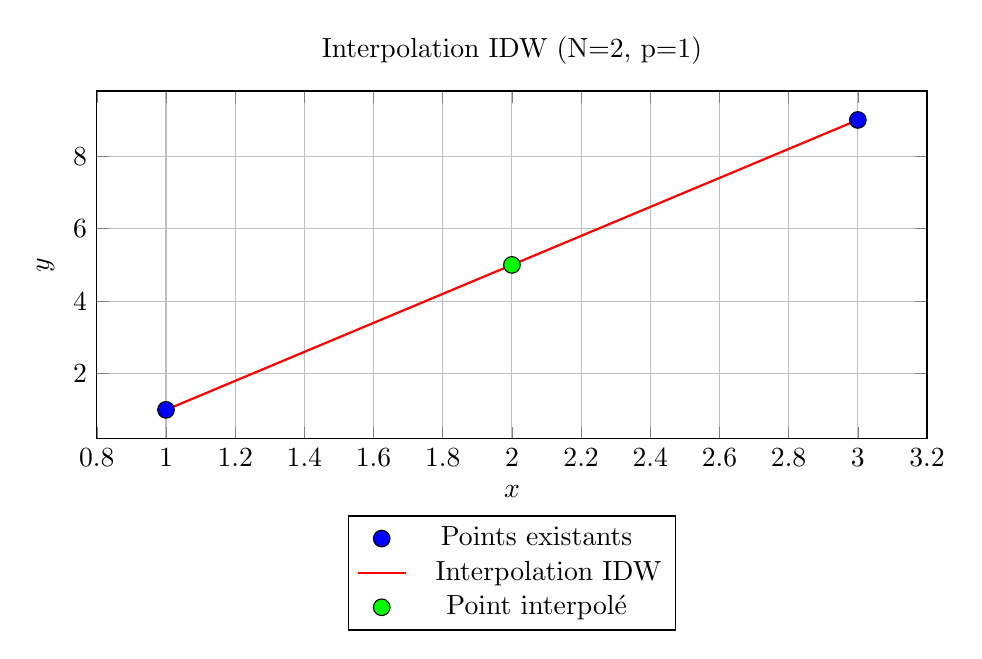
\begin{tikzpicture}
    \begin{axis}[
        width=\textwidth,
        height=6cm,
        title={Interpolation IDW (N=2, p=1)},
        xlabel={$x$},
        ylabel={$y$},
        grid=major,
        legend style={at={(0.5,-0.22)}, anchor=north, legend columns=1},
    ]
    \addplot[
        only marks,
        mark=*,
        mark options={scale=1.5, fill=blue},
    ] coordinates {
        (1, 1)
        (3, 9)
    };
    \addlegendentry{Points existants\hspace{0,3cm}}

    \addplot[
        domain=1:3,
        samples=100,
        smooth,
        thick,
        red,
    ] {(1/abs(1-x) + 9/abs(x-3))/(1/(abs(1-x))+1/(abs(x-3)))};
    \addlegendentry{\hspace{0,3cm}Interpolation IDW\hspace{0,3cm}}

    \addplot[
        only marks,
        mark=*,
        mark options={scale=1.5, fill=green},
    ] coordinates {
        (2, 5)
    };
    \addlegendentry{Point interpolé}
    \end{axis}
\end{tikzpicture}
\end{minipage}
\hspace{0.5cm}
\begin{minipage}{0.45\textwidth}
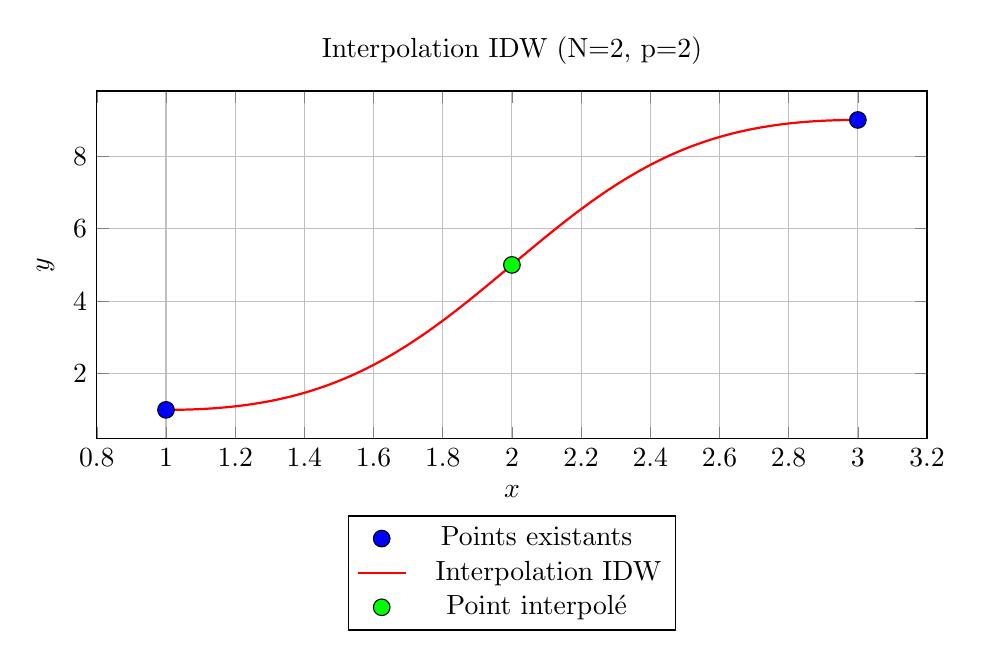
\begin{tikzpicture}
    \begin{axis}[
        width=\textwidth,
        height=6cm,
        title={Interpolation IDW (N=2, p=2)},
        xlabel={$x$},
        ylabel={$y$},
        grid=major,
        legend style={at={(0.5,-0.22)}, anchor=north, legend columns=1},
    ]
    \addplot[
        only marks,
        mark=*,
        mark options={scale=1.5, fill=blue},
    ] coordinates {
        (1, 1)
        (3, 9)
    };
    \addlegendentry{Points existants\hspace{0,3cm}}

    \addplot[
        domain=1:3,
        samples=100,
        smooth,
        thick,
        red,
    ] {(1/(abs(1-x)^2) + 9/(abs(x-3)^2))/(1/(abs(1-x)^2)+1/(abs(x-3)^2))};
    \addlegendentry{\hspace{0,3cm}Interpolation IDW\hspace{0,3cm}}

    \addplot[
        only marks,
        mark=*,
        mark options={scale=1.5, fill=green},
    ] coordinates {
        (2, 5)
    };
    \addlegendentry{Point interpolé}
    \end{axis}
\end{tikzpicture}
\end{minipage}
\end{center}

%\vspace{0.5cm}

\begin{center}
\begin{minipage}{0.45\textwidth}
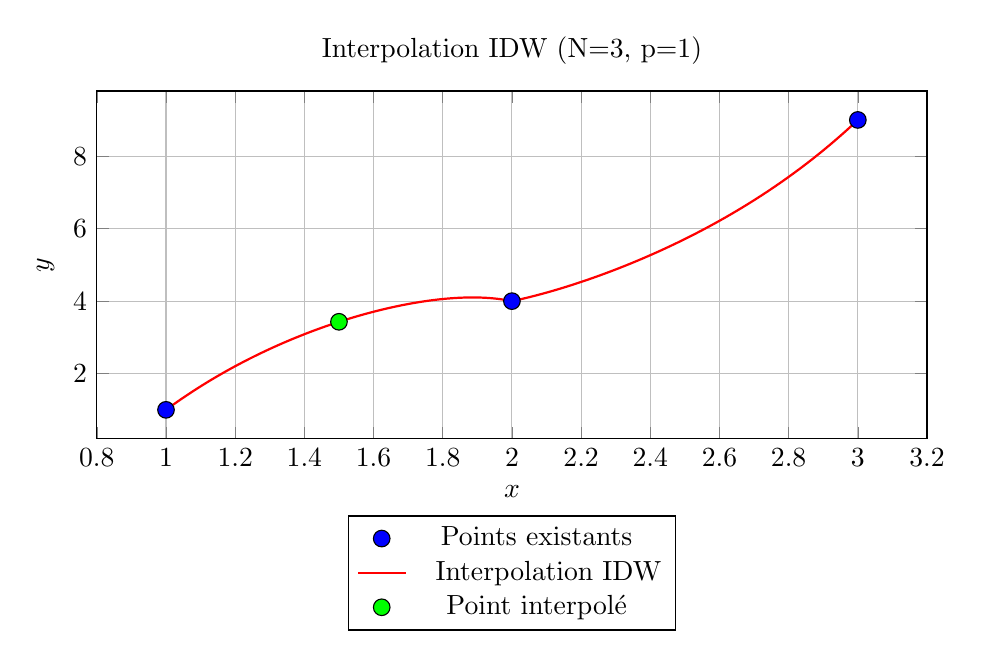
\begin{tikzpicture}
    \begin{axis}[
        width=\textwidth,
        height=6cm,
        title={Interpolation IDW (N=3, p=1)},
        xlabel={$x$},
        ylabel={$y$},
        grid=major,
        legend style={at={(0.5,-0.22)}, anchor=north, legend columns=1},
    ]
    \addplot[
        only marks,
        mark=*,
        mark options={scale=1.5, fill=blue},
    ] coordinates {
        (1, 1)
        (3, 9)
        (2, 4)
    };
    \addlegendentry{Points existants\hspace{0,3cm}}

    \addplot[
        domain=1:3,
        samples=100,
        smooth,
        thick,
        red,
    ] {(1/abs(1-x) + 9/abs(x-3) + 4/abs(2-x))/(1/(abs(1-x)) + 1/(abs(x-3)) + 1/(abs(2-x)))};
    \addlegendentry{\hspace{0,3cm}Interpolation IDW\hspace{0,3cm}}

    \addplot[
        only marks,
        mark=*,
        mark options={scale=1.5, fill=green},
    ] coordinates {
        (1.5, 3.43)
    };
    \addlegendentry{Point interpolé}
    \end{axis}
\end{tikzpicture}
\end{minipage}
\hspace{0.5cm}
\begin{minipage}{0.45\textwidth}
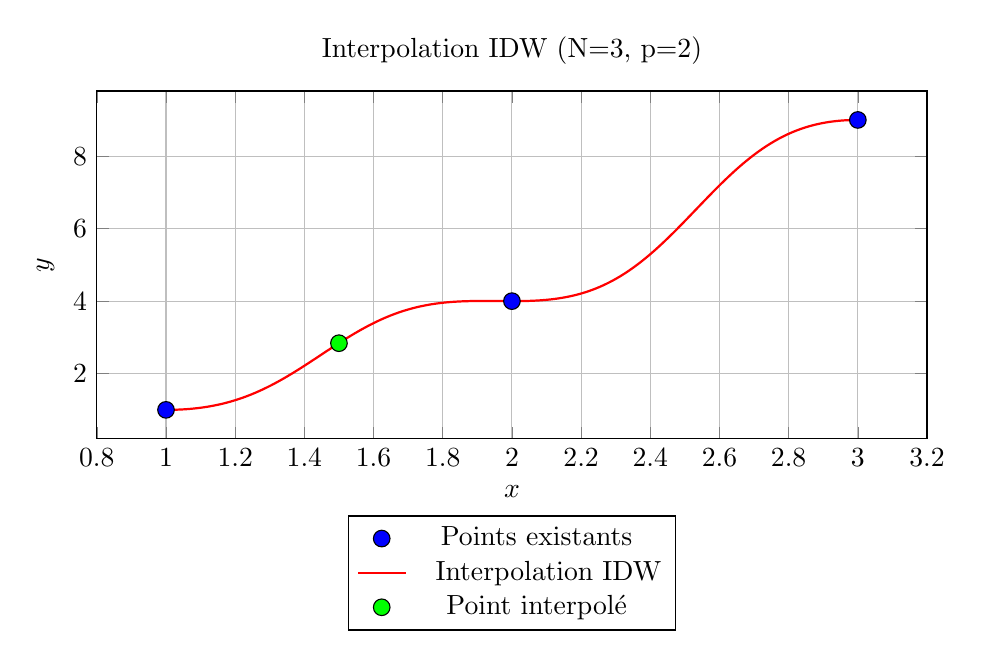
\begin{tikzpicture}
    \begin{axis}[
        width=\textwidth,
        height=6cm,
        title={Interpolation IDW (N=3, p=2)},
        xlabel={$x$},
        ylabel={$y$},
        grid=major,
        legend style={at={(0.5,-0.22)}, anchor=north, legend columns=1},
    ]
    \addplot[
        only marks,
        mark=*,
        mark options={scale=1.5, fill=blue},
    ] coordinates {
        (1, 1)
        (3, 9)
        (2, 4)
    };
    \addlegendentry{Points existants\hspace{0,3cm}}

    \addplot[
        domain=1:3,
        samples=100,
        smooth,
        thick,
        red,
    ] {(1/(abs(1-x)^2) + 9/(abs(x-3)^2) + 4/(abs(2-x)^2))/(1/(abs(1-x)^2) + 1/(abs(x-3)^2) + 1/(abs(2-x)^2))};
    \addlegendentry{\hspace{0,3cm}Interpolation IDW\hspace{0,3cm}}

    \addplot[
        only marks,
        mark=*,
        mark options={scale=1.5, fill=green},
    ] coordinates {
        (1.5, 2.84)
    };
    \addlegendentry{Point interpolé}
    \end{axis}
\end{tikzpicture}
\end{minipage}
\end{center}

%\vspace{0.5cm}

\begin{center}

\begin{tikzpicture}
    \begin{axis}[
        width=10cm,
        height=6cm,
        title={Interpolation IDW (N=3, p=2, rayon=1.5)},
        xlabel={$x$},
        ylabel={$y$},
        grid=major,
        legend style={at={(0.5,-0.22)}, anchor=north, legend columns=-1},
    ]
    \addplot[
        only marks,
        mark=*,
        mark options={scale=1.5, fill=blue},
    ] coordinates {
        (1, 1)
        (2, 4)
        (3, 9)
    };
    \addlegendentry{Points existants\hspace{0,5cm}}

    % Plotting the radius for the nearest neighbors
    \addplot[dashed, bronze, thick] coordinates {(1.5, 0) (1.5, 9)};
    \addlegendentry{Rayon de 1.5\hspace{0,3cm}}

    \addplot[
        domain=1:1.5,
        samples=100,
        smooth,
        thick,
        red,
    ] {(1/(abs(1-x)^2) + 4/(abs(x-2)^2))/(1/(abs(1-x)^2)+1/(abs(x-2)^2))};
    \addplot[
        domain=1.5:2.5,
        samples=100,
        smooth,
        thick,
        red,
    ] {(1/(abs(1-x)^2) + 9/(abs(x-3)^2) + 4/(abs(2-x)^2))/(1/(abs(1-x)^2) + 1/(abs(x-3)^2) + 1/(abs(2-x)^2))};
    \addplot[
        domain=2.5:3,
        samples=100,
        smooth,
        thick,
        red,
    ] {(4/(abs(x-2)^2) + 9/(abs(3-x)^2))/(1/(abs(x-2)^2)+1/(abs(3-x)^2))};
    \addlegendentry{Interpolation IDW}

    \addplot[dashed, bronze, thick] coordinates {(2.5, 0) (2.5, 9)};

    \end{axis}
\end{tikzpicture}
\end{center}

\vspace{0.5cm}

\begin{center}
    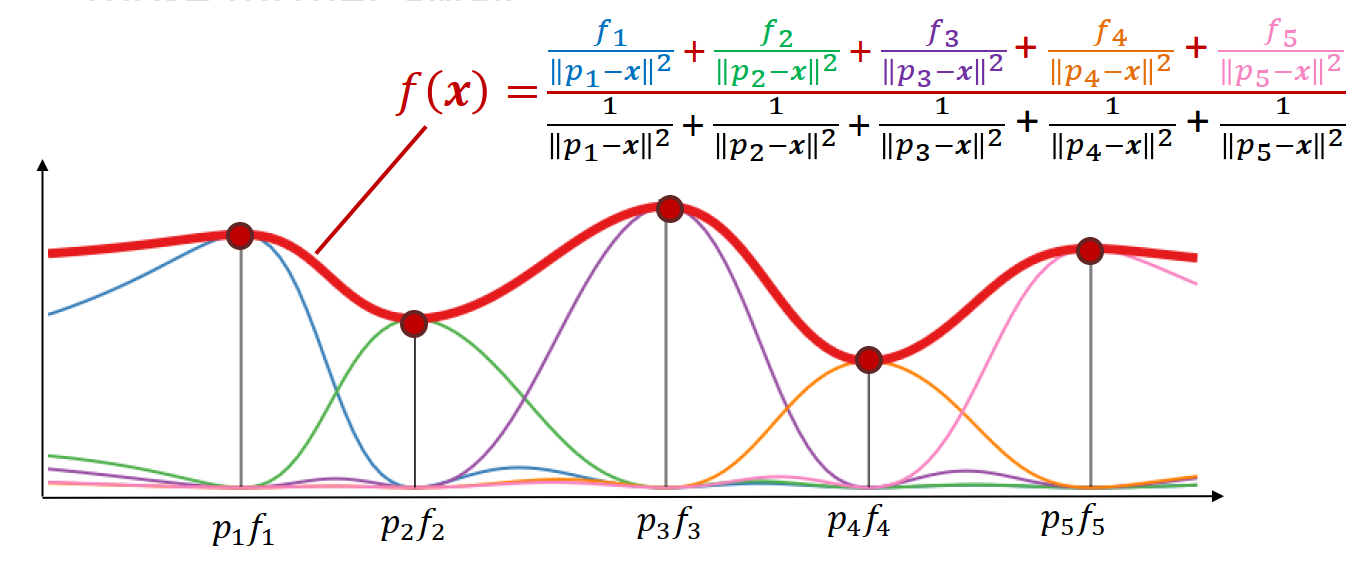
\includegraphics[width=0.8\textwidth]{images/Inverse_Distance_Weighting.png}
\end{center}


\begin{tikzpicture}
    \begin{axis}[
        view={0}{90},
        xlabel={$x$},
        ylabel={$y$},
        colorbar,
        title={Interpolation IDW en 2D (N=3, p=2, Rayon=2.0)},
        colormap/jet,
        width=12cm,
        height=10cm,
    ]

    % Points d'interpolation connus
    \pgfplotstableread{
        x y z
        1 1 1
        3 1 9
        2 3 4
    }\datatable

    % Fonction IDW
    \addplot3[
        surf,
        shader=interp,
        domain=0:4,
        y domain=0:4,
        samples=40,
    ] 
    {(1/(sqrt((x-1)^2+(y-1)^2)^2) + 
    9/(sqrt((x-3)^2+(y-1)^2)^2) + 
    4/(sqrt((x-2)^2+(y-3)^2)^2)) / 
    (1/(sqrt((x-1)^2+(y-1)^2)^2) + 
    1/(sqrt((x-3)^2+(y-1)^2)^2) + 
    1/(sqrt((x-2)^2+(y-3)^2)^2))}
     
    % Points d'interpolation connus
    \addplot3[
        only marks,
        scatter,
        scatter src=explicit,
        point meta=\thisrow{z},
        mark=square*,
        mark options={scale=2},
    ] table [x=x, y=y, z=z] {\datatable};

    % Annoter les points
    \node at (axis cs:1,1,1) [anchor=north] {A};
    \node at (axis cs:3,1,9) [anchor=north] {B};
    \node at (axis cs:2,3,4) [anchor=south] {C};

    \end{axis}
\end{tikzpicture}

Nous comprenons assez vite que, si nous définissons une distance à partir de laquelle nous prenons en compte ou non un point, cette méthode est discontinue.
Nous pouvons aussi imaginer que 2 points à droit et à gauche d'une ligne horizontale de 3 points (les plus proches), prendrons la même valeur pour \( N \) = 3, Schématiser. 

D'autres méthodes dérivées ou similaires existent pour évaluer nos poids. La plus intéressante serait celle dite de Franke-Littke. Elle consiste à utiliser une distance maximale autour du point au-delà les autres points ne sont pas pris en compte. Autrement dit, en utilisant un cercle (dans le cas 2D) d'un certain rayon pour déterminer quels points nous sont utiles pour l'interpolation. Dans ce cas le nombre de points est variable.
J'ai considéré subjectivement que cette méthode n'était pas intéressante car, confronté à un maillage ayant une différence de raffinement intrinsèque importante, dans certains cas aucuns points ne seraient pris, et dans d'autres, une grande somme serait calculée.

\begin{comment}
    Certaines conditions de cette méthode doivent être respectés, comme Pour N tends vers l’infini, p doit être inférieur ou égale à la dimension, par ex 3 pour ne pas diverger. Mais N n’est pas grand dans notre cas.
    Voir d'autres choses page 7 de mon ppt.
\end{comment}

Nous pouvons modifier 2 paramètres : \(p\) et \(N\).
Par défaut, dans le code, \(p\) = 1 et \(N\) est égale aux nombres de sommets de la première cellule de la liste de types de cellules de la base target. Il y aurait peut-être une modification mineure à faire sur ce point. La structure de la base target importe peu à côté de celle de la base source, pour l'interpolation. Mais aucune modification qui pourrait changer l'utilisation qui a déjà été faite de ce traitement ne pourra être faite par soucis de rétrocompatibilité. ! Tests à faire ici !



Nous remarquons que pour \( N = 1 \), nous retrouvons la méthode du voisin le plus proche, pour tout \( p \).
Et pour \( N = 2 \) et \( p = 1 \), toujours en 1D, nous retrouvons la méthode linéaire.

Une de mes missions étais de chercher s'il y avait des paramètres plus optimisés que \(N\) et \(p\) pour cette méthode. Je n'ai pas trouvé la réponse dans les différents articles et thèses que j'ai lues. C'est pour cela que je présenterais plus tard comment j'ai trouvé des paramètres optimaux en faisant des tests.


\subsection{L'interpolation polynomiale}
\subsection{L'interpolation par Splines}
\subsection{Méthodes géostatiques}
\subsection{Méthode par moindres carrés}
\subsection{MISCOG}

\subsection{L'interpolation linéaire}
L'interpolation linéaire, est la plus simple (après les plus proches voisins et IDW). Elle est moyennement précise et ne demande que peu de ressource. Elle interpole généralement mieux qu'IDW. C'est pour cela que le CERFACS voulait l'implémenter dans Antares. C'est aussi la plus utilisée par Airbus, Safran et d'autres industriels (dans via d'autres codes qu'Antares). Cela les arrange donc aussi d'avoir une interpolation linéaire directement dans Antares.

% Remplacer target par cible et point interpolé par cible.

\paragraph{1D}
\subparagraph{Linéaire}

En 1D, l'interpolation linéaire est simple : c'est la moyenne pondérée linéairement par la distance, des valeurs des points.
Supposons que nous voulons interpoler une valeur d'un point \( p \) entre deux points \( a \) et \( b \) dans un espace 1D
et que nous représentons leurs valeurs dans une deuxième dimension \( y \).
Nous aurons alors pour formule :

\[
y_p = \frac{x_b - x_p}{x_b - x_a} \cdot y_a + \frac{x_p - x_a}{x_b - x_a} \cdot y_b
\]

%\vspace*{0.1\baselineskip}\linebreak
où \( y_p \) représente la valeur interpolée à la position \( x_p \), et \((x_a, y_a)\) et \((x_b, y_b)\) sont les points de référence. J'ai écrit cette formule afin qu'elle soit symétrique par rapport aux points \( a \) et \( b \), pour qu'ils jouent la même rôle. Ainsi elle s'entendra plus intuitivement dans des dimensions supérieures.
\vspace{0.5cm}
%\vspace*{0.1\baselineskip}\linebreak

        \( \frac{x_b - x_p}{x_b - x_a} \) est le poids pour \( y_a \) basé sur la distance relative de \( x_p \) à \( x_b \).

        \( \frac{x_p - x_a}{x_b - x_a} \) est le poids pour \( y_b \) basé sur la distance relative de \( x_p \) à \( x_a \).\vspace{0.5cm}

Ces deux termes sont pondérés de manière que leur somme soit toujours égale à 1, ce
qui garantit que l'interpolation est correcte et symétrique par rapport à \( a \) et \( b \).\vspace{0.5cm}


\paragraph{2D}

En 2D, nous devons nous baser sur des surfaces, extraites de formes pour pouvoir effectuer cette pondération. En CFD, ces formes sont appelées cellules et leurs sommets nœuds. Dans notre cas, nous considérons que les variables du maillage sont contenus au niveau des nœuds. Aussi, Antares ne traites que des maillages ayant des valeurs uniquement au niveau des nœuds des cellules (pas entre).
Il existe 3 principaux types de cellules (formes) en 2D : les triangles 'tri', et les quadrilatères 'qua' (non croisés) et les rectangles des maillages structurés (dans ce cas, la méthode est dite bilinéaire).

\subparagraph{Triangle : Barycentrique}

Pour le triangle, la méthode pour trouver la valeur au point à interpoler \( p \) est celle dite du barycentre (barycentrique).
Elle est bien documentée. Visuellement, il faut faire la somme des valeurs aux points pondérés par la surface opposés et pondéré le tout par la surface du triangle.

\begin{comment}
    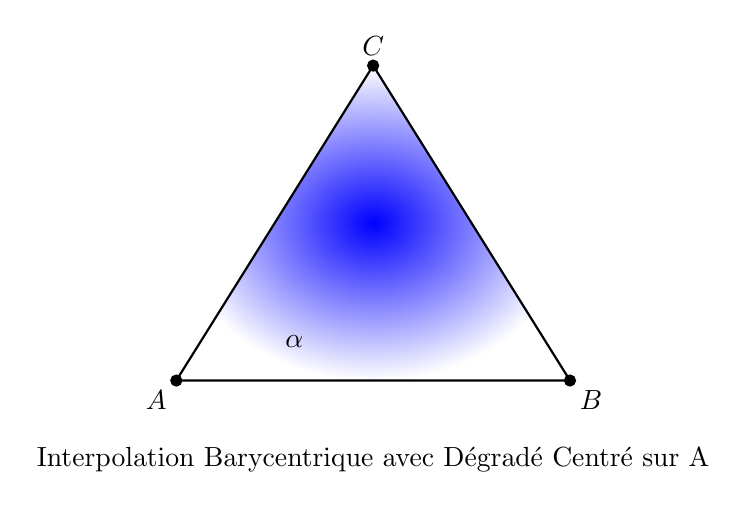
\begin{tikzpicture}
    % Triangle coordinates
    \coordinate (A) at (0,0);
    \coordinate (B) at (5,0);
    \coordinate (C) at (2.5,4);

    % Gradient fill centered at vertex A
    \shade[shading=radial, inner color=blue, outer color=white] (A) -- (B) -- (C) -- cycle;

    % Draw triangle
    \draw[thick] (A) -- (B) -- (C) -- cycle;

    % Draw labels and points
    \filldraw[black] (A) circle (2pt) node[anchor=north east] {$A$};
    \filldraw[black] (B) circle (2pt) node[anchor=north west] {$B$};
    \filldraw[black] (C) circle (2pt) node[anchor=south] {$C$};
    \node at (1.5,0.5) {$\alpha$};

    % Title
    \node at (2.5,-1) {Interpolation Barycentrique avec Dégradé Centré sur A};

\end{tikzpicture}
\end{comment}

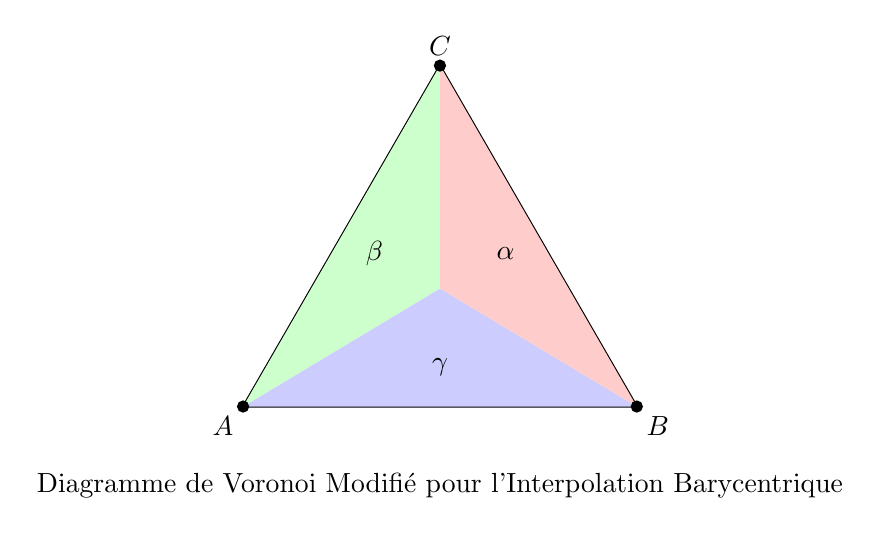
\begin{tikzpicture}

    % Define the triangle vertices
    \coordinate (A) at (0,0);
    \coordinate (B) at (5,0);
    \coordinate (C) at (2.5,4.33);
    \coordinate (P) at (2.5,1.5); % Point d'interpolation

    % Draw triangle
    \draw[thick] (A) -- (B) -- (C) -- cycle;

    % Draw Voronoi-like regions
    \fill[blue!20]  (A) -- (B) -- (P) -- cycle;
    \fill[red!20]   (B) -- (C) -- (P) -- cycle;
    \fill[green!20] (C) -- (A) -- (P) -- cycle;
    %\fill[green!20] (C) -- (barycentric cs:A=1,B=0,C=1) -- (barycentric cs:A=0,B=1,C=1) -- cycle;

    % Draw points
    \filldraw[black] (A) circle (2pt) node[anchor=north east] {$A$};
    \filldraw[black] (B) circle (2pt) node[anchor=north west] {$B$};
    \filldraw[black] (C) circle (2pt) node[anchor=south] {$C$};

    % Add labels
    \node at (barycentric cs:B=1,C=1,P=1) {$\alpha$};
    \node at (barycentric cs:C=1,A=1,P=1) {$\beta$};
    \node at (barycentric cs:A=1,B=1,P=1) {$\gamma$};

    % Title
    \node at (2.5,-1) {Diagramme de Voronoi Modifié pour l'Interpolation Barycentrique};

\end{tikzpicture}

% Trilinéaire dans le cas où le maillage est 3D et structuré.
\subparagraph{Rectangle : bilinéaire}

En ce qui concerne l'interpolation bilinéaire sur un rectangle, nous la trouvons aussi facilement. La formule est l'extension de celle pour les triangles :

ÉQUATION

Visuellement nous créons cette fois des traits parallèles au passant par le point d'interpolation et nous additionnons, de manière pondérée, les 4 surfaces multipliées chacune par leur sommet opposé respectif. Cela correspond à deux interpolations linéaires. Souvent nous trouvons une équation analytique où tous les sommets ne jouent pas le même rôle, mais je trouvais cela plus simple de faire un calcul de poids pour pouvoir ensuite faire une moyenne pondérée :

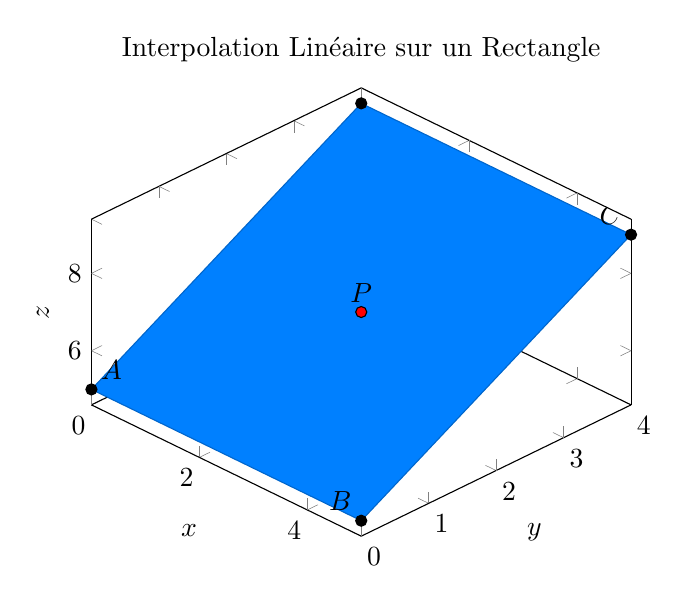
\begin{tikzpicture}
    \begin{axis}[
        view={45}{45},
        xlabel={$x$},
        ylabel={$y$},
        zlabel={$z$},
        colormap/cool,
        title={Interpolation Linéaire sur un Rectangle},
        ]

        % Define the vertices of the rectangle
        \addplot3[surf, mesh/rows=2, domain=0:5, domain y=0:4] 
            coordinates {(0,0,5) (5,0,5) (0,4,9) (5,4,9)};

        % Draw points for vertices and their labels
        \addplot3[only marks, mark=*] coordinates {(0,0,5) (5,0,5) (5,4,9) (0,4,9)};
        \addplot3[only marks, mark=*, mark options={fill=red}] coordinates {(2.5,2,7)};

        % Labels for the vertices and interpolated point
        \node at (axis cs:0,0,5) [anchor=south west] {$A$};
        \node at (axis cs:5,0,5) [anchor=south east] {$B$};
        \node at (axis cs:5,4,9) [anchor=south east] {$C$};
        \node at (axis cs:0,4,9) [anchor=south west] {$D$};
        \node at (axis cs:2.5,2,7) [anchor=south] {$P$};

    \end{axis}
\end{tikzpicture}



ILLUSTRATION

\subparagraph{Quadrilatère}

Viens maintenant la dernière forme 2D rencontrée dans les solutions traités par Antares : les quadrilatères. Pour cela je n'ai pas trouvé de méthode. Après plusieurs essais sur papier, je me suis concentré sur le fait que la méthode devait être continue, ce qui implique notamment que la valeur du point à interpoler doit tendre vers la valeur d'un sommet lorsque sa distance à ce dernier tend vers 0. Une première vérification de la linéarité est aussi de vérifier qu'un point au milieu d'une forme 2D a comme valeur la moyenne de ses côtés.
Via cette démarche, j'ai imaginé, graphiquement, tracer des traits entre le point à interpoler et les sommets de la forme dans laquelle il se situe (tel que pour l'interpolation Barycentrique). Cela permet de ne créer uniquement 4 sous formes. Ensuite pour déterminer le poids associé au sommet \( s_1 \), il faut multiplier les deux surfaces qui lui sont opposés entre elles, et bien entendu, le pondéré une fois les autres poids calculés. Par opposé j'entends que ces surfaces ne sont composés d'aucune arrête ayant pour l'une de leurs extrémités le point d'interpolation. Ceci est important pour le 3D. Pour l'instant, je n'ai démontré que par l'expérimentation que cette méthode étais linéaire. Un point qui me perturbait étais de faire des multiplications de surfaces, donc ordre 4, dans une méthode linéaire. Mais contrairement à son nom, l'interpolation bilinéaire est en réalité quadratique avec un résultat linéaire. On pourrait imaginer que, par chance, ma méthode soit quadratique. Premièrement j'ai vérifié et ce n'est apparemment pas le cas. Deuxièmement je pense que le quadratique n'englobe pas le linéaire dans le cas où nous nous basons uniquement sur les quatre points d'un quadrilatère. Effectivement, en 1D, si nous avons \(f(x_i)\) = 0 et \(f(x_{i+1})\) = 1, le résultat d'une variable linéaire serait 0,5 et celui d'une variable quadratique 0,25, si nous avons uniquement connaissance de ces deux points. Normalement il faut s'appuyer sur plus de points pour le quadratique. Finalement voici l'équation :\\
ÉQUATION

ILLUSTRATION\vspace{0.5cm}  % OU \\[0pt plus 1fill] OU \newline OU flushleft, flushright, center


\paragraph{3D}
\subparagraph{Pavé droit : Trilinéaire}

Pour le 3D, si le maillage est structuré, alors la forme est le pavé droit. À ce moment, nous sommes dans le cas de l'interpolation dite trilinéaire. Encore une fois la formule se trouve facilement. Nous associons comme poids à un des huit sommets \( s_1 \) le volume opposé, construit de la sorte :

\begin{figure}[ht!]
    \centering
    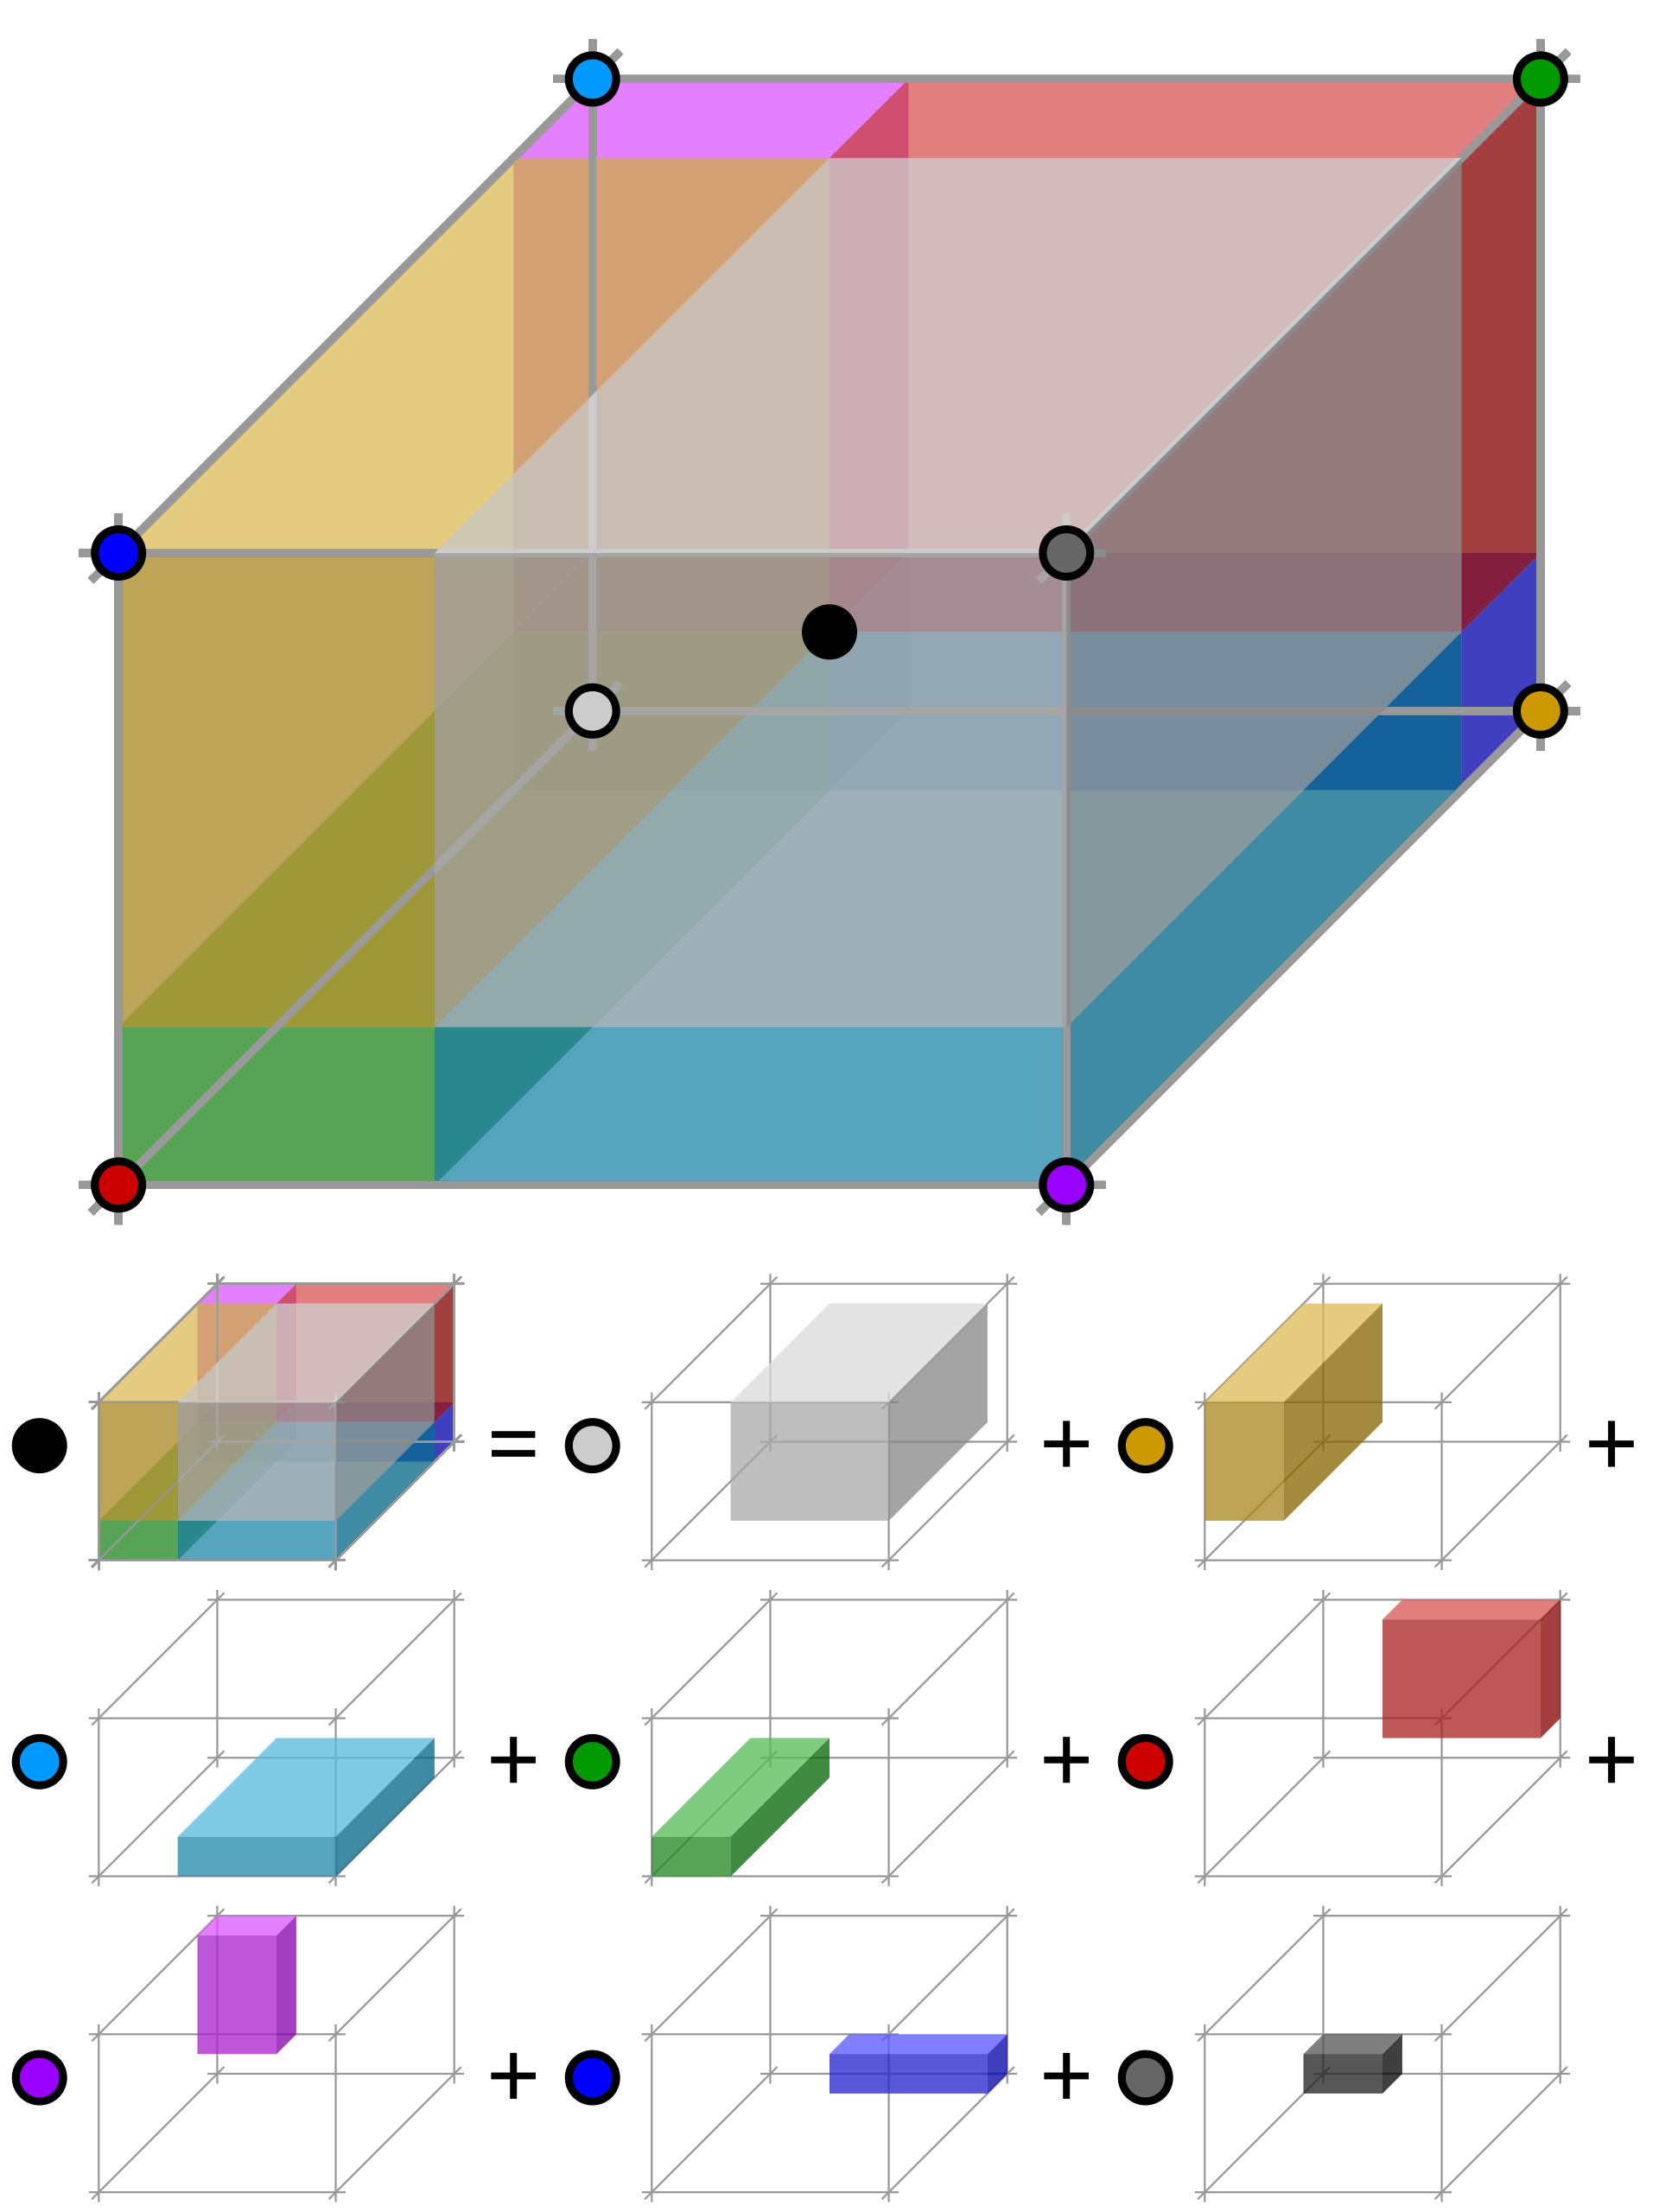
\includegraphics[width=0.4\textwidth]{images/Trilinear_interpolation_visualisation.svg.png}
    \caption{Interpolation trilinéaire} %\footnote{Source:https://en.wikipedia.org/wiki/Trilinear_interpolation#/media/File:Trilinear_interpolation_visualisation.svg}}
    %\label{fig:https://en.wikipedia.org/wiki/Trilinear_interpolation#/media/File:Trilinear_interpolation_visualisation.svg}
\end{figure}

L'équation qui en découle est la suivante :

\begin{equation}
    f(x, y, z) = \sum_{i=0}^{1} \sum_{j=0}^{1} \sum_{k=0}^{1} f_{ijk} (1 - |x - x_i|)(1 - |y - y_j|)(1 - |z - z_k|)
\end{equation}

% Expliquer mathématiquement ? Ou plus tard dans le code ?  (quadrilatère non croisé, concave et convexes)

% En CFD il y a toujours des formes, même si c'est structuré, on peut unstructure.

\subsection{Résumé des similitudes et différences des différentes méthodes}



\section{Mission 2 : Implémenter la méthode trilinéaire}
\subsection{La structure générale du code TreatmentInterpolation}
Après avoir recensé les différentes méthodes qui seraient applicables, ma seconde mission a été d'implémenter une interpolation linéaire dans Antares. Grâce à Nitrox, j'ai accès au code source de la librairie que je peux modifier. Le code 'interpolation.py' faisais environ 500 lignes. Il est orienté objet. Il prend comme arguments obligatoires la base source et la base target et renvoie dans le cas le plus simple la base target avec les valeurs interpolés.
De manière simplifiée, dans le code, les zones de la base source sont fusionnées puis nous parcourons les instants. 
Cette fusion permet de faire un KDTree (pour arbre à k-dimensions), qui permet concrètement de rechercher de manière efficace quels sont les \( N \) points de la base source les plus proches des points de la base target (et les distances associées, utilisés dans la méthode 'idw').

Ensuite nous calculons l'interpolation via une méthode 'principale' (\lstinline{__idw_interpolate_instant} ou
\lstinline{__barycentrique_interpolate_instant}) qui peut elle-même appeler des fonctions ou méthodes.

\subsection{L'algorithme}
Si vraiment ce n'est pas confidentiel je peux mettre le code en annexe Carlos.

Premièrement, dans \lstinline{__barycentrique_interpolate_instant}, nous récupérons le nombre de points maximal sur lequel nous allons nous appuyer pour l'interpolation, soit le nombre maximal de sommet des formes présentes dans le maillage.
Nous récupérons les distances et indices du KDTree.
Ensuite nous devons réarranger des indices qui se sont fait déplacer lors de la fusion des zones.
Nous récupérons aussi différentes variables, comme les coordonnées des points, \dots

%Nous récupérons d'une fonction définie plus bas (\lstinline{get_list_cell_type}) :
%(\lstinline{list_cell_type, max_node_index})


Dans le cas où le maillage est le même entre tous les instants, nous ne recalculons pas tous ces paramètres, ce qui permet une diminution significative du temps de calcul.


%Expliquer 'is point on cell', etc...


%\subsection{La prise en main de la libraire Antares}
\subsection{...}

EXEMPLE DE MISE EN FORME PYTHON
\begin{lstlisting}[caption=Calcul de l'interpolation, label={lst:interpolation}]
    def __idw_interpolate_instant(x, y, z, values, power=2):
        # Calculer l'interpolation IDW
        weights = [(1 / (distance**power)) for distance in distances]
        interpolated_value = sum(w * v for w, v in zip(weights, values)) / sum(weights)
        return interpolated_value
    
    def __barycentrique_interpolate_instant(x, y, z, values):
        # Calculer l'interpolation barycentrique
        weights = [barycentric_weight(x, y, z, vertex) for vertex in vertices]
        interpolated_value = sum(w * v for w, v in zip(weights, values))
        return interpolated_value
\end{lstlisting}


\subsection{Les difficultés}
\subsection{Le résultat}



\section{Mission 3 : Tester sur des cas d'aéroacoustique}
% \section{Les différentes méthodes d'interpolation}
Carlos a développé l'outil permettant de déterminer le résultat acoustique, à grande distance, à partir d'une surface, en utilisant les équations de Ffowcs Williams – Hawkings. Le résultat acoustique sont les petites variations de pression, impliquant du son (à différentes fréquences et amplitudes). En pratique, pour les utilisateurs d'Antares, cette surface est définie dans un maillage 'solution' où nous avons le résultat de la pression en différents points et différents instants.
% Paramètres d'IDW
\subsection{Tests sur les paramètres de la méthode IDW}




... (\url{https://cerfacs.fr/antares/}) : 


\begin{itemize}
    \item TreeMesh 
    %Ici, le maillage DGMultiMesh dépend directement du solver DGMulti en fonction du type de géométrie utilisée, il faut donc le passer en argument.
\end{itemize}


\subsection{Discrétisation spatiale et résolution du problème}